%!TeX root=../viewsbodytop.tex
\addchap{Solution to the Puzzle in <Uncle Meleager's Will>}

{\scshape\Large\bfseries Notes to the Solution}

\def\arraystretch{1.5}
	
\begin{longtable} {c p{0.8\linewidth}} 
	
\textsc{i}.1. & \textsc{virgo}: The sign of the zodiac between \textsc{leo} (strength) and \textsc{libra} (justice). Allusion to parable of The Ten Virgins.\\

\textsc{i}.3. & \textsc{r.s.}: Royal Society, whose <fellows> are addicted to studies usually considered dry-as-dust.\\

\textsc{iv}.3. & \textsc{testament} (or will); search is to be directed to the Old Testament. Ref. to parable of New Cloth and Old Garment.\\

\textsc{xiv}.3. & \textsc{hi}:
\begin{verse}
He would answer to Hi!\\
Or to any loud cry.
\end{verse}
\textit{The Hunting of the Snark.}\\

\textsc{i}.5. & \textsc{trans}.: Abbreviation of Translation; ref. to building of Babel.\\

\textsc{xi}.5. & \textsc{scent}:
\begin{verse}
Even the scent of roses\\
Is not what they supposes,\\
But more than mind discloses\\
And more then men believe.\\
\end{verse}
\textit{G.~K. Chesterton: The Song of Quoodle.}\\

\textsc{vi}.7. & \textsc{ictus}: Blow; add V (five) and you get \textsc{victus} (vanquished); the ictus is the stress in a foot of verse; if the stress be misplaced the line goes lamely.\\

\textsc{i}.8. & \textsc{spinoza}: He wrote on the properties of optical glasses; also on metaphysics.\\

\textsc{iv}.13. & \textsc{thirty-one}: Seven (months) out of the twelve of the sun's course through the heavens have thirty-one days.\\

\textsc{xiv}.13. & \textsc{et}: Conjunction. In astrology an aspect of the heavenly bodies. That Cicero was the master of this word indicates that it is a Latin one.\\

\textsc{x}.14. & \textsc{bezoar}: The bezoar stone was supposed to be a prophylactic against poison.\\

11.\textsc{i.} & \textsc{plaud}: If you would laud, then plaud (var. of applaud); Plaud-it also means <cheer.>\\

10.\textsc{ii.} &  \textsc{aliena}: \textit{As You Like It}. \textsc{II}.1.130.\\

1.\textsc{iii.} &  \textsc{r.d.}: <Refer to Drawer.>\\

4.\textsc{iii.} &  \textsc{canticles}: The Magnificat and Nunc Dimittis are known as the Canticles, but the Book of Canticles (the Vulgate name for the Song of Songs, in which the solution is found) occurs earlier in the Bible.\\

2.\textsc{vi.}. &  \textsc{est}: ὀν και μη ὀν [Greek: 'on kai mê 'on] = \textit{est and non est}—the problem of being and not-being. Ref. Marlowe: \textit{Doctor Faustus} \textsc{I}.1.\\

12.\textsc{x.} &  \textsc{tob}.: Add \textsc{it} to get Tobit; the tale of Tobit and the Fish is in the Apocrypha (the book of hidden things).\\

1.\textsc{xi.} &  \textsc{manes}: <Un lion est une mâchoire et non pas une crinière>: Emile Faguet: \textit{Lit. du \textsc{XVII}\textsuperscript{e} siècle}. Manes: benevolent spirits of the dead.\\

1.\textsc{xv}. &  \textsc{saint}: Evidence of miraculous power is required for canonisation.\\
\end{longtable}

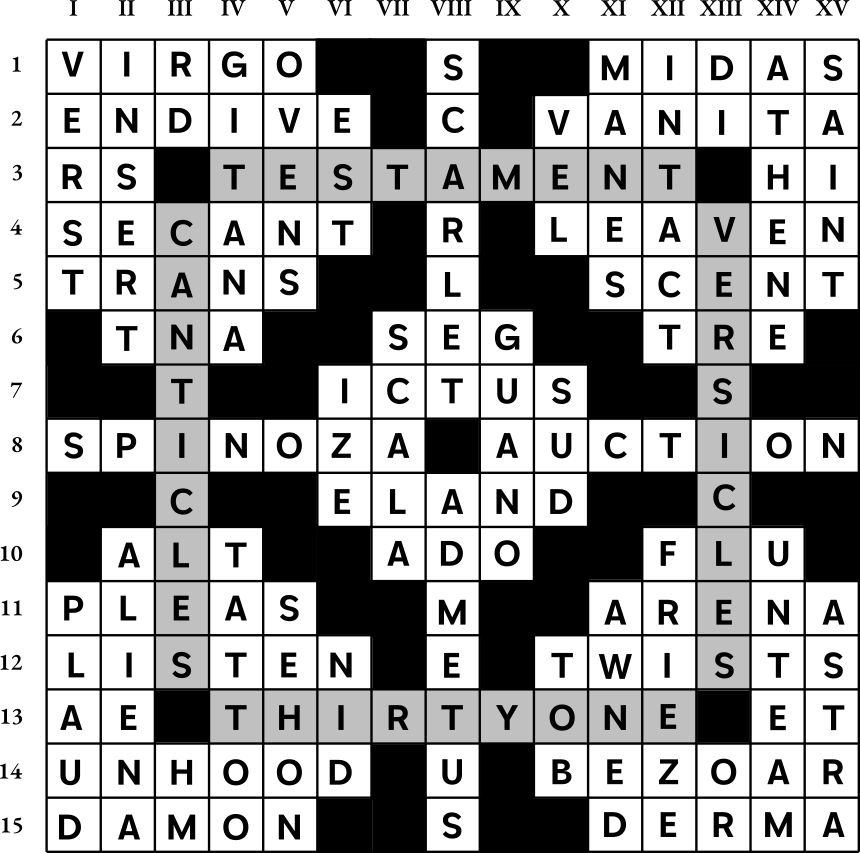
\includegraphics[width=\textwidth]{puzzlesolved}